\section{Espacios proyectivos}

\begin{definición}[Espacio proyectivo]
Dado un espacio vectorial $V$ se define el espacio proyectivo o el proyectivizado de $V$ y se denota por $\mathbb{P}(V)$ como el conjunto de rectas vectoriales de $V$.\\
A momentos nos olvidaremos de $V$ y llamaremos $\mathbb{P} = \mathbb{P}(V)$ espacio proyectivo.
\end{definición}

\begin{definición}[Dimension de un espacio proyectivo]
Si $V$ es un espacio vectorial, se define la dimensión del espacio proyectivo $\mathbb{P}(V)$ como:
\[    dim(\mathbb{P}(V)) = dim(V) - 1 \]
\end{definición}

\ejemplo{
    Si $V$ es un espacio vectorial de $dim=1$ (una recta vectorial) entonces todos los vectores de $V$ son proporcionales y por tanto $V$ solo tiene una recta vectorial. Por tanto $\mathbb{P}(V)$ es un punto y $dim(\mathbb{P}(V))=dim(V)$.
}

\begin{observación}
Los subespacios generados por un vector y por todos sus proporcionales son el mismo subespacio, por ejemplo:\\
$$ L[\vec{u}] = L[\vec{-2u}]$$
\begin{center}
    \begin{tikzpicture}[scale=1.2]
        % Ejes coordenados
        \draw[->, gray] (0,0,0) -- (2.5,0,0) node[anchor=west] {$x$};
        \draw[->, gray] (0,0,0) -- (0,2.5,0) node[anchor=south] {$y$};
        \draw[->, gray] (0,0,0) -- (0,0,2.5) node[anchor=north east] {$z$};
        % Recta generada por u menos inclinada
        \draw[<->, gray!60] (-2.5, -1.25, -0.625) -- (2.5, 1.25, 0.625) node[anchor=south east] {Recta $\langle u \rangle$};
        % Vector u = (2,1,0.5)
        \draw[->, thick, blue] (0,0,0) -- (1,0.5,0.25) node[anchor=west] {$u$};
        % Vector -2u = (-2,-1,-0.5)
        \draw[->, thick, red] (0,0,0) -- (-2,-1,-0.5) node[anchor=east] {$-2u$};
    \end{tikzpicture}
\end{center}
\end{observación}

\ejemplo{
    Si $V = \{\vec{0}\}$ entonces $\mathbb{P}(V) = \emptyset$ y $dim(\mathbb{P}(V)) = dim(V) - 1 = 0 - 1 = -1$.
}

\begin{observación}
Pensaremos salvo que se diga lo contrario que el cuerpo de coeficientes de $V$ es $\mathbb{K} = \mathbb{R}$ ó $\mathbb{K} = \mathbb{C}$.
\end{observación}

\begin{definición}[Espacio proyectivo canónico]
Se llama espacio proyectivo canónico sobre $\mathbb{K}$ de dimension $n$ al proyectivizado de $\mathbb{K}^{n+1}$.\\
Se denotaran por $\mathbb{P}^n(\mathbb{R})$ y $\mathbb{P}^n(\mathbb{C})$ respectivamente.\\
Otras notaciones habituales son $\mathbb{R}\mathbb{P}^n$ y $\mathbb{C}\mathbb{P}^n$, ó $\mathbb{P}^n(\mathbb{R})$ y $\mathbb{P}^n(\mathbb{C})$.
\end{definición}

\begin{definición}[Definicion alternativa de espacio proyectivo]
Podemos definir el espacio proyectivo como:
$$ \mathbb{P}(V) = \frac{V \setminus \{\vec{0}\}}{\sim} $$
Donde $\sim$ es la relación de equivalencia definida como:
$$ \vec{u} \sim \vec{v} \iff \exists \lambda \in \mathbb{K}^* : \vec{u} = \lambda \vec{v} $$
Es decir, dos vectores son equivalentes si son proporcionales.
\end{definición}

\begin{definición}[Subespacio proyectivo]
Dado $\mathbb{P} = \mathbb{P}(V)$ un espacio proyectivo, llamaremos subespacios proyectivos (a veces subvariedades o variedades proyectivas) de $\mathbb{P}$ a los subconjuntos de la forma $\mathbb{P}(W)$ donde $W$ es un subespacio vectorial de $V$.
\end{definición}

\ejemplo{

    \begin{itemize}
        \item Pongamos de ejemplo los subespacios degenerados:\\
        $\{\vec{0}\}$, $V$ son subespacios vectoriales de $V$ y por tanto $\mathbb{P}(\{\vec{0}\}) = \emptyset$ y $\mathbb{P}(V) = \mathbb{P}$ son subespacios proyectivos de $\mathbb{P}$.
        \item Si $\mathbb{P}=\mathbb{P}(V)$ es un espacio proyectivo de dimensión 3 ($\dim(V)=4$).
    \end{itemize}

\begin{center}
    \renewcommand{\arraystretch}{1.3}
    \begin{tabular}{|c|c|c|}
        \hline
        $\dim(W)$ & Subespacios vectoriales de $V$ & Subespacios proyectivos de $\mathbb{P}$                  \\
        \hline
        $dim = 4$ & $V$                            & $\mathbb{P} = \mathbb{P}(V)$ con $\dim = dim(V) - 1 = 3$ \\
        $dim = 3$ & Hiperplanos vectoriales        & Planos proyectivos con $\dim = 2$                                      \\
        $dim = 2$ & Planos vectoriales             & Rectas proyectivas con $\dim = 1$                                      \\
        $dim = 1$ & Rectas vectoriales             & Puntos proyectivos con $\dim = 0$                                      \\
        $dim = 0$ & $\{\vec{0}\}$                  & $\emptyset$ con $dim = -1$                               \\
        \hline
    \end{tabular}
\end{center}

}



\observacion{
    A los subespacios proyectivos de codimension 1 (es decir, de $dim = dim(\mathbb{P}) - 1$) se les llama hiperplanos proyectivos.
}

\begin{lema}
    Dados dos puntos distintos $A$ y $B$ de un espacio proyectivo $\mathbb{P}$ existe una recta que los contiene.
    $$ A=[\vec{u}], B=[\vec{v}]$$
    La recta que los contiene es:
    $$ r = \mathbb{P}(W) \ \text{con} \ W = L[\vec{u}, \vec{v}] $$
    Donde $dim(W) = 2$, $\vec{u}$ y $\vec{v}$ son independientes porque $A \neq B$.
    Asi $r = \mathbb{P}(W)$ es una recta proyectiva que contiene a $A$ y $B$.

    % Ejemplo visual: dos puntos proyectivos y la recta que los contiene
    \begin{center}
        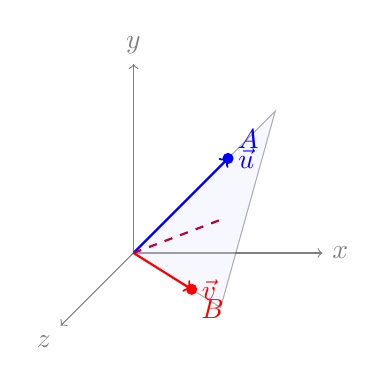
\begin{tikzpicture}[scale=1.2]
            % Ejes coordenados
            \draw[->, gray] (0,0,0) -- (2,0,0) node[anchor=west] {$x$};
            \draw[->, gray] (0,0,0) -- (0,2,0) node[anchor=south] {$y$};
            \draw[->, gray] (0,0,0) -- (0,0,2) node[anchor=north east] {$z$};
            % Plano generado por u y v
            \filldraw[fill=blue!10, opacity=0.3] (0,0,0) -- (1.5,1.5,0) -- (1.5,0,1.5) -- cycle;
            % Vector u
            \draw[->, thick, blue] (0,0,0) -- (1,1,0) node[anchor=west] {$\vec{u}$};
            % Vector v
            \draw[->, thick, red] (0,0,0) -- (1,0,1) node[anchor=west] {$\vec{v}$};
            % Punto A
            \filldraw[blue] (1,1,0) circle (1.5pt) node[anchor=south west] {$A$};
            % Punto B
            \filldraw[red] (1,0,1) circle (1.5pt) node[anchor=north west] {$B$};
            % Recta proyectiva (intersección de plano y espacio)
            \draw[thick, purple, dashed] (0,0,0) -- (1.2,0.6,0.6);
        \end{tikzpicture}
    \end{center}
\end{lema}

\begin{proposición}[Propiedades de espacios proyectivos]
    Sea $\mathbb{P} = \mathbb{P}(V)$ un espacio proyectivo de dimensión $n$.
    \begin{itemize}
        \item $\mathbb{P}$ envia todos los subespacios vectoriales de $V$ en subespacios proyectivos de $\mathbb{P}$.
        \item $\mathbb{P}$ es sobreyectiva.
        \item $\mathbb{P}$ es inyectiva, es decir, $\mathbb{P}(W_1) = \mathbb{P}(W_2) \iff W_1 = W_2$.
        \item Si $W_1 \subseteq W_2 \implies \mathbb{P}(W_1) \subseteq \mathbb{P}(W_2)$.
    \end{itemize}
\end{proposición}

\begin{proposición}[Intersección de subespacios proyectivos]
    Dados $\{X_i : i \in I\}$ subespacios proyectivos de $\mathbb{P} = \mathbb{P}(V)$, entonces su intersección $\bigcap_{i \in I} X_i$ es un subespacio proyectivo de $\mathbb{P}$.\\
\end{proposición}

\begin{proof}
    Tenemos que probar que $\bigcap_{i \in I} X_i = P(W)$ donde $W$ es un subespacio vectorial de $V$.\\
    Por hipótesis, $X_i = \mathbb{P}(W_i)$ donde $W_i$ es un subespacio vectorial de $V$.\\
    Veamos por tanto que $\bigcap_{i \in I} X_i = \mathbb{P}(\bigcap_{i \in I} W_i)$, siendo este ultimo un subespacio vectorial de $V$ al ser intersección de subespacios vectoriales.\\
    Cada elemento de $\bigcap_{i \in I} X_i$ es una recta vectorial que pertenece a todos los $X_i$, es decir, a todos los $\mathbb{P}(W_i)$, luego esta contenida en todos los $W_i$ y por tanto en $\bigcap_{i \in I} W_i$.\\
\end{proof}

\begin{definición}[Subespacio generado]
    Sea $S \subseteq \mathbb{P} = \mathbb{P}(V)$ un subconjunto, se define el subespacio proyectivo generado por $S$, y se denota por $V(S)$ como el menor subespacio proyectivo que contiene a $S$.\\
\end{definición}

\begin{proof}
    Veamos que la definicion tiene sentido, es decir que $V(S)$ existe y es único, definiendolo de la siguiente manera:
    \[
    V(S) = \bigcap_{\substack{X \subseteq \mathbb{P} \\ S \subseteq X}} X
    \]
    Este conjunto es no vacío porque $\mathbb{P}$ es un subespacio proyectivo contenido en $\mathbb{P}$ y contiene a $S$.\\
    Evidentemente $S \subset \bigcap_{\substack{X \subseteq \mathbb{P} \\ S \subseteq X}} X$, y la intersección es un subespacio proyectivo por la proposición anterior, y si no fuera el menor estaríamos intersecando también el menor.\\
    En el caso en que $S$ es la unión de subespacios proyectivos (puntos, rectas, planos, etc) $X_1, X_2, \ldots, X_k$, el subespacio generado se denota por $V(X_1, X_2, \ldots, X_k)$ ó $X_1 + X_2 + \ldots + X_k$.
\end{proof}

\ejemplo{
    Sean $A,B$ dos puntos distintos de un espacio proyectivo $\mathbb{P}$, sabemos que $\exists r : A,B \in r$ la recta proyectiva que los contiene, siendo esta el menor subespacio proyectivo que contiene a $A$ y $B$, es decir:
    \[
    r = V(A,B) = A + B
    \]
    \begin{center}
    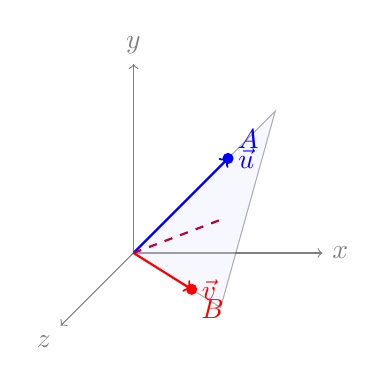
\begin{tikzpicture}[scale=1.2]
        % Ejes coordenados
        \draw[->, gray] (0,0,0) -- (2,0,0) node[anchor=west] {$x$};
        \draw[->, gray] (0,0,0) -- (0,2,0) node[anchor=south] {$y$};
        \draw[->, gray] (0,0,0) -- (0,0,2) node[anchor=north east] {$z$};
        % Plano generado por u y v
        \filldraw[fill=blue!10, opacity=0.3] (0,0,0) -- (1.5,1.5,0) -- (1.5,0,1.5) -- cycle;
        % Vector u
        \draw[->, thick, blue] (0,0,0) -- (1,1,0) node[anchor=west] {$\vec{u}$};
        % Vector v
        \draw[->, thick, red] (0,0,0) -- (1,0,1) node[anchor=west] {$\vec{v}$};
        % Punto A
        \filldraw[blue] (1,1,0) circle (1.5pt) node[anchor=south west] {$A$};
        % Punto B
        \filldraw[red] (1,0,1) circle (1.5pt) node[anchor=north west] {$B$};
        % Recta proyectiva (intersección de plano y espacio)
        \draw[thick, purple, dashed] (0,0,0) -- (1.2,0.6,0.6);
    \end{tikzpicture}
    \end{center}
}

\begin{observación}[Formula de Grassmann para espacios proyectivos]
    Si $X_1, X_2$ son subespacios proyectivos de $\mathbb{P}$ entonces:
    \[
    \dim(X_1 \cap X_2) + \dim(V(X_1, X_2)) = \dim(X_1) + \dim(X_2)
    \]
\end{observación}

\begin{proof}
    Sean $X_1 = \mathbb{P}(W_1)$ y $X_2 = \mathbb{P}(W_2)$, entonces:\\
    \[
    X_1 \cap X_2 = \mathbb{P}(W_1 \cap W_2) = V(X_1, X_2) = \mathbb{P}(L[W_1, W_2])
    \]
    Esta ultima igualdad se puede generalizar como:
    \[
    V(X_1, X_2 \ldots, X_k) = \mathbb{P}(L[W_1, W_2, \ldots, W_k])
    \]
    Por la fórmula de Grassmann (vectorial) sabemos que:
    \[
    \dim(W_1 \cap W_2) + \dim(L[W_1, W_2]) = \dim(W_1) + \dim(W_2) \iff
    \]
    \[
    \dim(X_1 \cap X_2) + \dim(V(X_1, X_2)) = \dim(X_1) + \dim(X_2) \iff
    \]
    \[
    \dim(W_1 \cap W_2) - 1 + \dim(L[W_1, W_2]) - 1 = \dim(W_1) - 1 + \dim(W_2) - 1 
    \]
\end{proof}

